\documentclass[12pt]{article}
\usepackage[utf8]{inputenc}
\usepackage{amsmath}
\usepackage{graphicx}
\graphicspath{ {./} }
\setlength{\parskip}{1em}

\title{Week 4 Questions}
\author{tprasad@tcd.ie 16326505}
\pagenumbering{gobble}
\begin{document}
\maketitle
\begin{flushleft}
Question 1

	(a) \{(1,1)\}
	
	(b)	\{(2,1),(1,2)\}
	
	(c)	\{(1,3),(3,1),(2,2)\}
	
	(d) \[ \frac{3}{6^2} = 0.08333 \] since 3 events and a total sample space of $6^2 $ different events
	
Question 2

	(a)	-3,-1,1,3 \newline
		If all tails then X = -1 -1 -1 = -3
		If one heads then X = -1 -1 +1 = -1
		Similarly we can get X for all possible outcomes after three flips
	
	(b) \[ \{(T,T,T)\} \]
	Are the events corresponding to X = -3 hence given $2^3$ different possible events
	\[ P(X = -3) = \frac{1}{2^3} = 0.125 \]
	
	(c) Using a similar logic as (b) above
	\[\{(H,T,T),(T,H,T),(T,T,H)\} = 0.375\]
	
	(d)	Probability of P(X=1) = P(X=-1) and  P(X=3) = P(X=-3)
	
	PMF = plotting out these values =
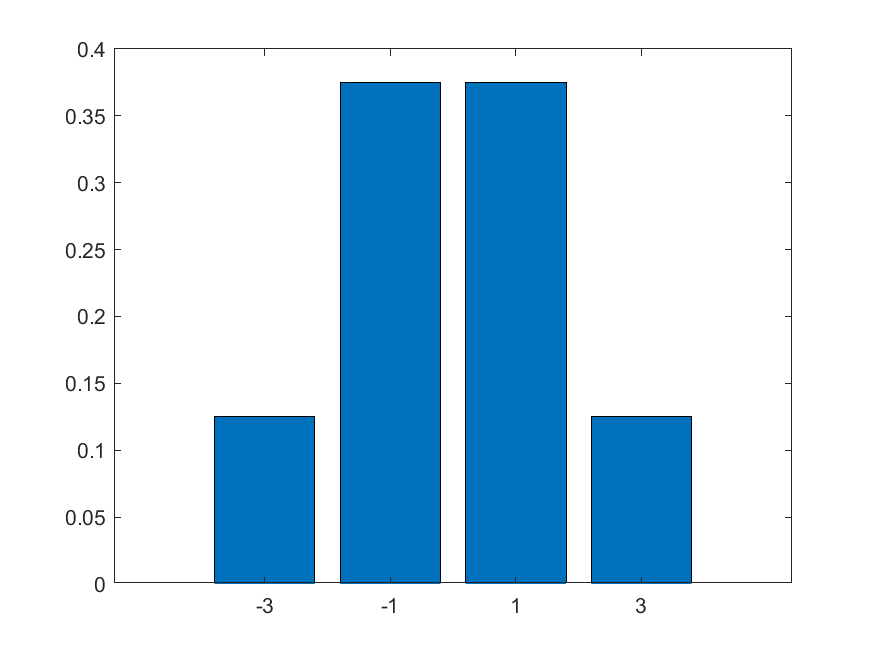
\includegraphics[scale=1]{PMF}

	CDF =
		\[ P(X = -3) = .125 \]
		\[ P(X = -1) = .375 + .125 = .5\]
		\[ P(X = 1) = .875 \]
		\[ P(X = 3) = 1 \]
		
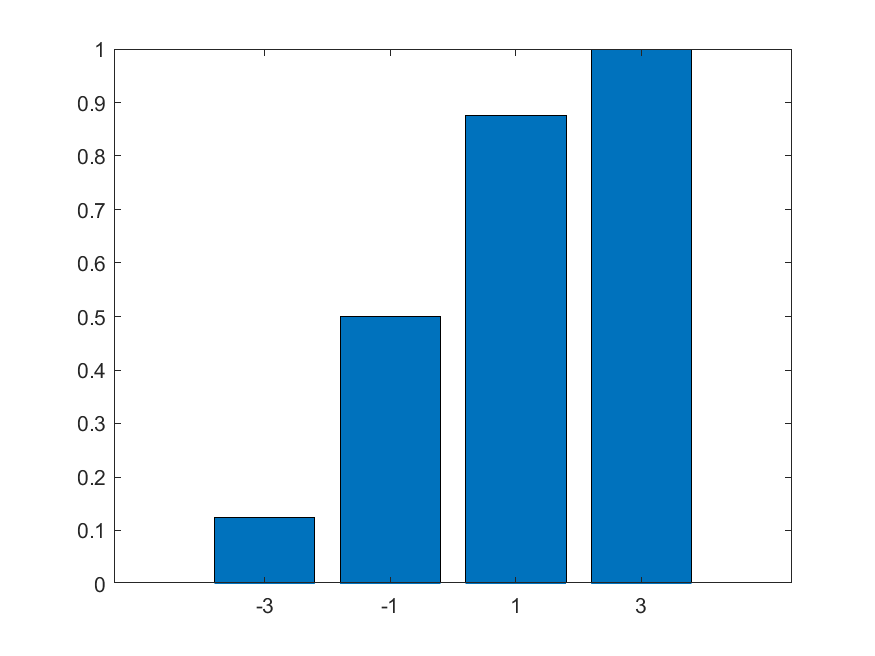
\includegraphics[scale=1]{Barchart}
		
	
		
Question 3

	(a) 1 since all numbers on the dice are $>= 1$
	
	(b) Exactly 1 possibility in 6 can't be landed on all 4 times, since if the die rolls a 1 then X = 1.
	\[ \left(\frac{5}{6}\right)^4 = 0.4823 \]
	
	(c)	$P(X<=k)$ for all k. 
		\[P(X<=1) \] can be derived through counting and summing up the following:
		\[ \binom{4}{1}*\left(\frac{5}{6}\right)^3*\left(\frac{1}{6}\right)^1  = \frac{125}{324}\]
		 \[ \binom{4}{2}*\left(\frac{5}{6}\right)^2*\left(\frac{1}{6}\right)^2 = \frac{25}{216}\]
		 \[ \binom{4}{3}*\left(\frac{5}{6}\right)^1*\left(\frac{1}{6}\right)^3 = \frac{5}{324}\]
		\[  \binom{4}{4}*\left(\frac{5}{6}\right)^0*\left(\frac{1}{6}\right)^4 = \frac{1}{1296}\]
		\[ P(X<=1) = \frac{671}{1296} \]
		
		\[P(X<=2) = P(X<=1) + P(X=2) \]
		\[ P(X<=1) = \frac{671}{1296} \]
		\[ \binom{4}{1}*\left(\frac{4}{6}\right)^3*\left(\frac{1}{6}\right)^1  = \frac{16}{81}\]
		 \[ \binom{4}{2}*\left(\frac{4}{6}\right)^2*\left(\frac{1}{6}\right)^2 = \frac{2}{27}\]
		 \[ \binom{4}{3}*\left(\frac{4}{6}\right)^1*\left(\frac{1}{6}\right)^3 = \frac{1}{81}\]
		\[  \binom{4}{4}*\left(\frac{4}{6}\right)^0*\left(\frac{1}{6}\right)^4 = \frac{1}{1296}\]
		\[ P(X<=2)= \frac{65}{81} \]
		...All these answers so far are correct but I have been enlightened as to just get 1 - (chance of not getting  any roll $<= X$) 
		\[ P(X<=3)=\frac{15}{16} \]
		\[  P(X<=4)=\frac{80}{81} \]
		\[  P(X<=5)=\frac{1295}{1296} \]
		\[  P(X<=6)=1 \]

	
\end{flushleft}
\end{document}